\documentclass[]{beamer}
\usepackage[utf8]{inputenc}
\usepackage[T1]{fontenc}
\usepackage{carlito}
\usetheme[horizontal=true, hr=false, pagenumbers=true]{NewPwr}
\usepackage{bibentry}
\usepackage{minted}
\setminted{fontsize=\small,baselinestretch=1}
\usepackage{multicol}
\usepackage{polski}

% Build-specific command
\nonstopmode

%Information to be included in the title page:
\title{Applied Observability}
\subtitle{Prognozy i trendy rozwojowe w informatyce}
\author{Mateusz Bączek}
\institute{Politechnika Wrocławska}
\date{2023}

\begin{document}

\frame{\titlepage}

\section{Wstęp teoretyczny}

\begin{frame}
\frametitle{Definicja problemu}
% \vspace{-1cm}
\begin{multicols}{2}
  \begin{enumerate}
    \item Tworzymy produkt,
    \item uruchamiamy produkt (na sprzęcie dedykowanym/w chmurze/na sprzęcie klienta),
    \item \textbf{czy produkt \textit{działa}?}
  \end{enumerate}

  \begin{figure}
    \centering
    
\includegraphics[width=0.8\linewidth]{elastic_search_banner.png}
    % \caption{Grafika reklamowa firmy \textit{Elastic}, tworzącej rozwiązania monitorujące.}
  \end{figure}
\end{multicols}

\end{frame}

\begin{frame}
\frametitle{Uszczegółowienie problemu}
\vspace{-1cm}

Co to znaczy, że nasz produkt \textbf{działa}?

\begin{enumerate}
  \item Czy produkt działa \textbf{w tej chwili}?
  \item Czy wystąpiły awarie \textbf{w przeszłości}?
  \item Czy sprawność działania produktu jest \textbf{stała w czasie}?
  \item Jakie metryki oceniają \textbf{sprawność działania produktu}?
  \item Czy wdrożono procedury, które należy podjąć w przypadku \textbf{wystąpienia awarii}?
\end{enumerate}
\end{frame}

\begin{frame}
  \frametitle{A gdy już zdaży się awaria?}

  \vspace{-1cm}
  \begin{itemize}
    \item Powiadomienie o wystąpieniu awarii,
    \item automatyczne restartowanie usług,
    \item automatyczne przywracanie backupów,
    \item automatyczne cofanie aktualizacji (\textit{rollback}),
    \item \textbf{analiza przyczyn wystąpienia awarii}.
  \end{itemize}
\end{frame}

\begin{frame}
  \frametitle{Co monitorujemy? \cite{gartner}} 

  \vspace{-1cm}
  \begin{enumerate}
    \item Infrastrukturę:
      \begin{itemize}
        \item serwery,
        \item chmurę,
        \item sieć.
      \end{itemize}
    \item Aplikacje:
      \begin{itemize}
        \item interfejsy użytkownika.
        \item bazy danych,
        \item interfejsy API.
      \end{itemize}
    \item Funkcje biznesowe:
      \begin{itemize}
        \item zdarzenia domenowe w systemie.
      \end{itemize}
  \end{enumerate}
\end{frame}

\begin{frame}
  \frametitle{\textit{Observability} jako standardowy element infrastruktury projektowej}
  \begin{figure}
    \centering
    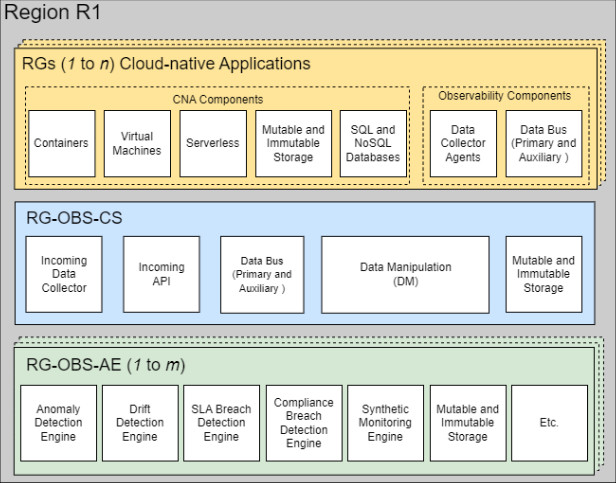
\includegraphics[width=0.6\linewidth]{cloud_architecture_proposal.jpg}
    \caption{Rekomendowana struktura aplikacji chmurowej opracowana przez specjalistów z uniwersytetów w Toronto oraz Maryland, we współpracy z IBM \cite{ibm}.}
  \end{figure}
\end{frame}

\begin{frame}
  \frametitle{Jakie są źródła danych dla systemu monitorującego?}
  \begin{enumerate}
    \item Logi generowane przez usługi,
    \item metryki pobierane z usług,
    \item zdarzenia (\textit{events}) emitowane przez system.
  \end{enumerate}
\end{frame}

\begin{frame}
  \frametitle{Od monitoringu do \textit{applied observability}}

  % \quote{https://www.gartner.com/smarterwithgartner/how-to-start-an-it-monitoring-initiative}
  % \quote{By 2021, 60% of IT monitoring investments will include a focus on business-relevant metrics, up from less than 20\% in 2017.}
  \begin{quote}
    By 2021, 60\% of IT monitoring investments will include a focus on business-relevant metrics, up from less than 20\% in 2017.
    \cite{gartner2}
  \end{quote}

  \begin{itemize}
    \item \textbf{zdecentralizowana} infrastruktura,
    \item coraz większy \textbf{koszt} \textit{downtime}'u,
    \item użytkownicy przyzwyczajeni do \textbf{ciągłej} dostępności usługi,
    \item większa moc urządzeń mobilnych - możliwość \textbf{monitorowania urządzeń klienckich},
    \item wykorzystywanie sztucznej inteligencji do \textbf{wykrywania anomalii},
    \item metryki jako obiektywne źródło danych przy \textbf{podejmowaniu decyzji} technicznych/biznesowych.
  \end{itemize}
\end{frame}

\section{Prosty przykład praktyczny}

\begin{frame}[fragile]
  \frametitle{Bardzo niski koszt wprowadzenia \textit{observability}}

  \vspace{-0.2cm}
  \begin{minted}{python}
from prometheus_client import start_http_server, Summary

app = Flask(__name__)
REQUEST_TIME = Summary(
    "request_processing_seconds",
    "Time spent processing request"
)

@app.route("/endpoint")
@REQUEST_TIME.time()
def example_endpoint():
    print("Processing a request..")
    time.sleep(random.randrange(1, 10))
    print("Processing finished!")
    return "Hello, world!"
  \end{minted}
\end{frame}

\begin{frame}
  \frametitle{Po konfiguracji w systemie \textit{Prometheus}}

  \begin{figure}
    \centering
    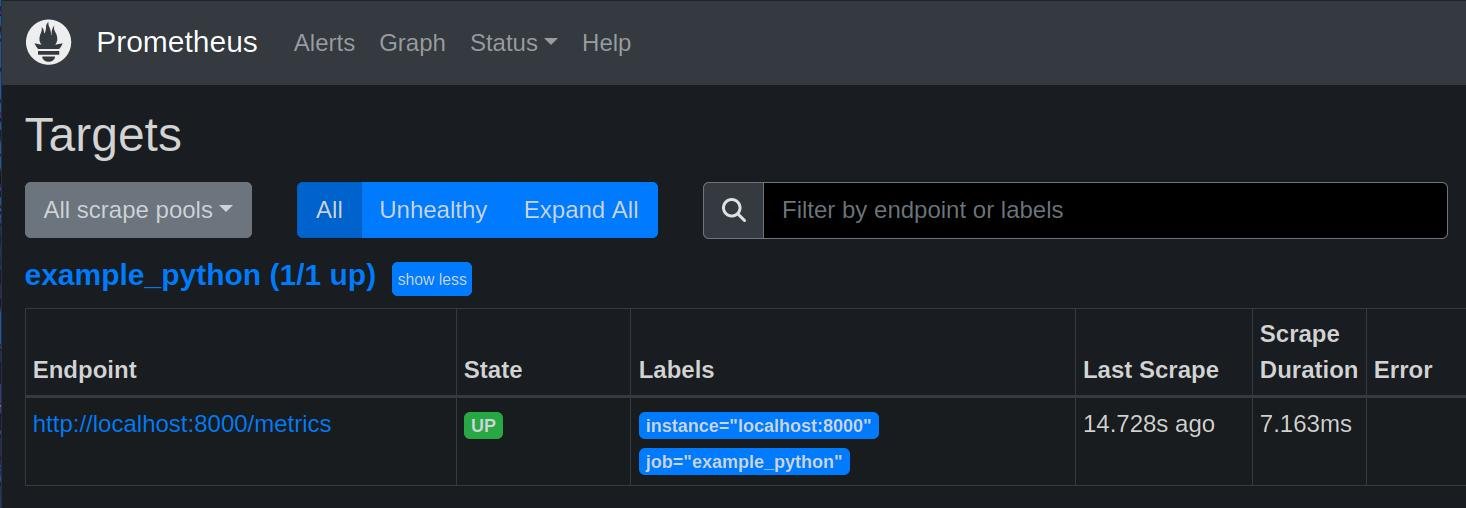
\includegraphics[width=0.7\linewidth]{prometheus_scrape_example.jpg}
    \caption{Status usługi w systemie \textit{Prometheus}.}
  \end{figure}

  \vspace{-0.5cm}

  \begin{figure}
    \centering
    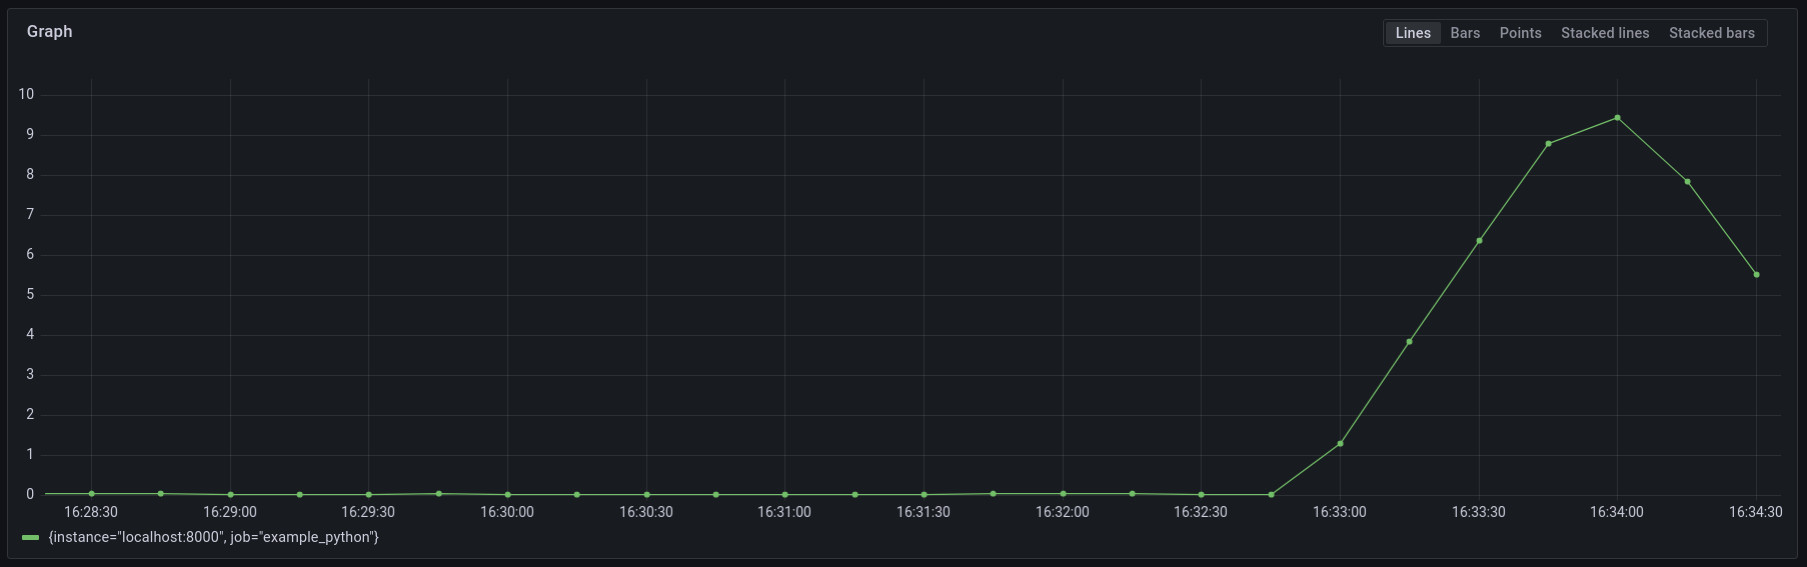
\includegraphics[width=0.7\linewidth]{grafana_example_python_monitoring.jpg}
    \caption{Wykres metryki \texttt{increase(process\_cpu\_seconds\_total)}}
  \end{figure}
\end{frame}

\section{Przegląd popularnych narzędzi}

\begin{frame}
  \frametitle{Popularne rozwiązania do monitorowania infrastruktury IT}
  \begin{figure}
    \centering
    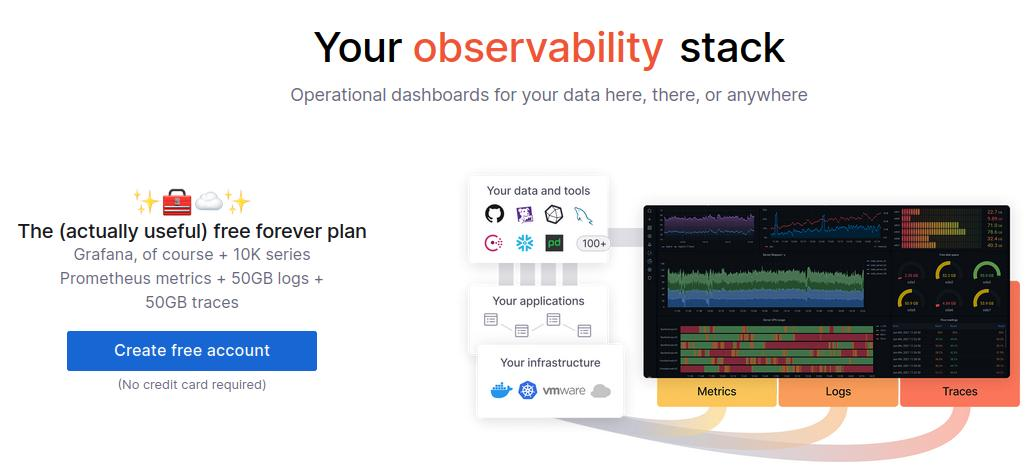
\includegraphics[width=0.8\linewidth]{grafana_website.jpg}
    \caption{Grafana -- wizualizacja danych z wielu źródeł, system alertowania.}
  \end{figure}
\end{frame}

\begin{frame}
  \frametitle{Popularne rozwiązania do monitorowania infrastruktury IT}
  \begin{figure}
    \centering
    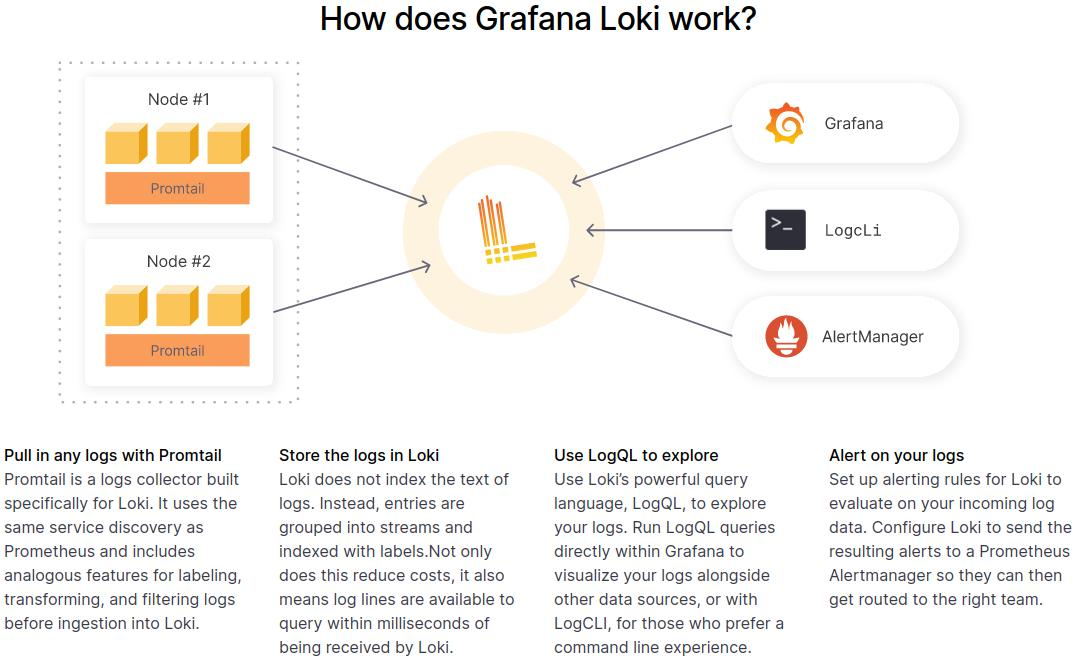
\includegraphics[width=0.8\linewidth]{loki.jpg}
    \caption{Loki -- centralne repozytorium logów.}
  \end{figure}
\end{frame}


\begin{frame}
  \frametitle{Popularne rozwiązania do monitorowania infrastruktury IT}
  \begin{figure}
    \centering
    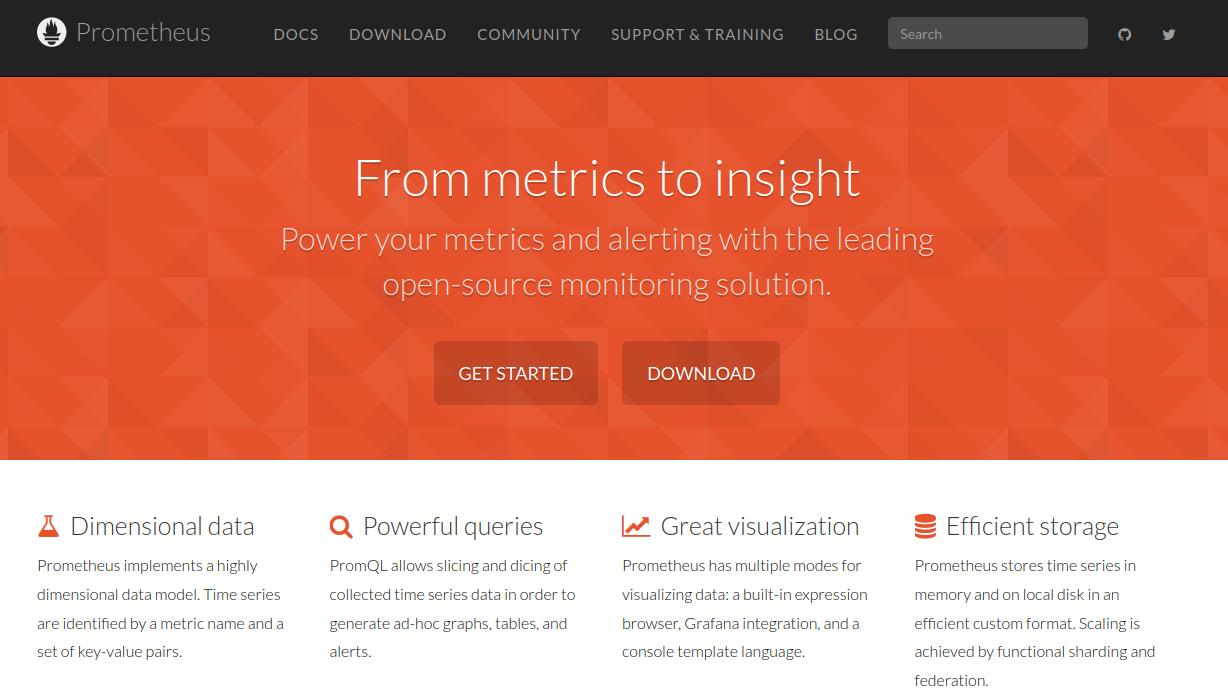
\includegraphics[width=0.8\linewidth]{prometheus.jpg}
    \caption{Prometheus -- narzędzie do zbierania i monitorowania metryk systemów informatycznych.}
  \end{figure}
\end{frame}


\begin{frame}
  \frametitle{Popularne rozwiązania do monitorowania infrastruktury IT}
  \begin{figure}
    \centering
    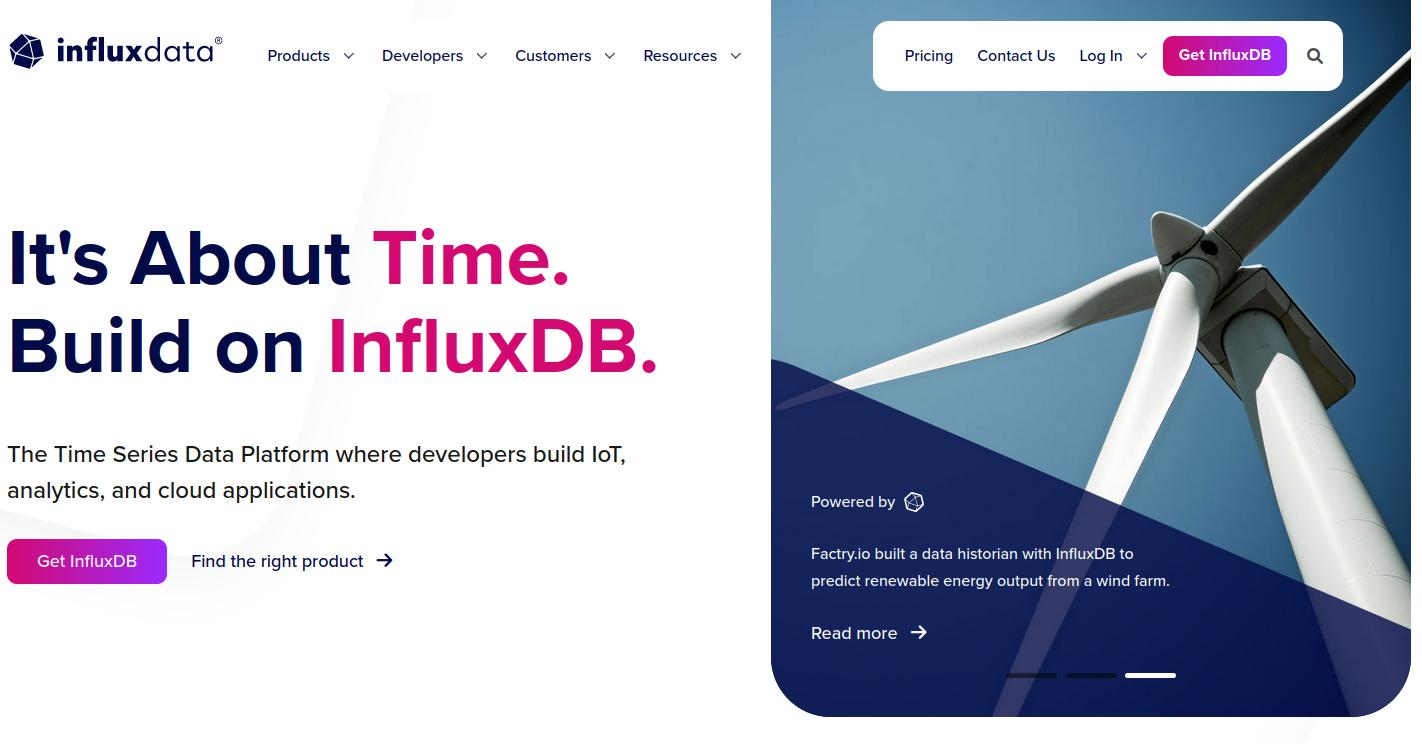
\includegraphics[width=0.9\linewidth]{influxdb.jpg}
    \caption{InfluxDB -- baza danych dedykowana do przechowywania danych pomiarowych.}
  \end{figure}
\end{frame}

\section{Monitorowanie własnej infrastruktury}

\begin{frame}
  \frametitle{Przykład -- monitorowanie własnej infrastruktury}
  \begin{figure}
    \centering
    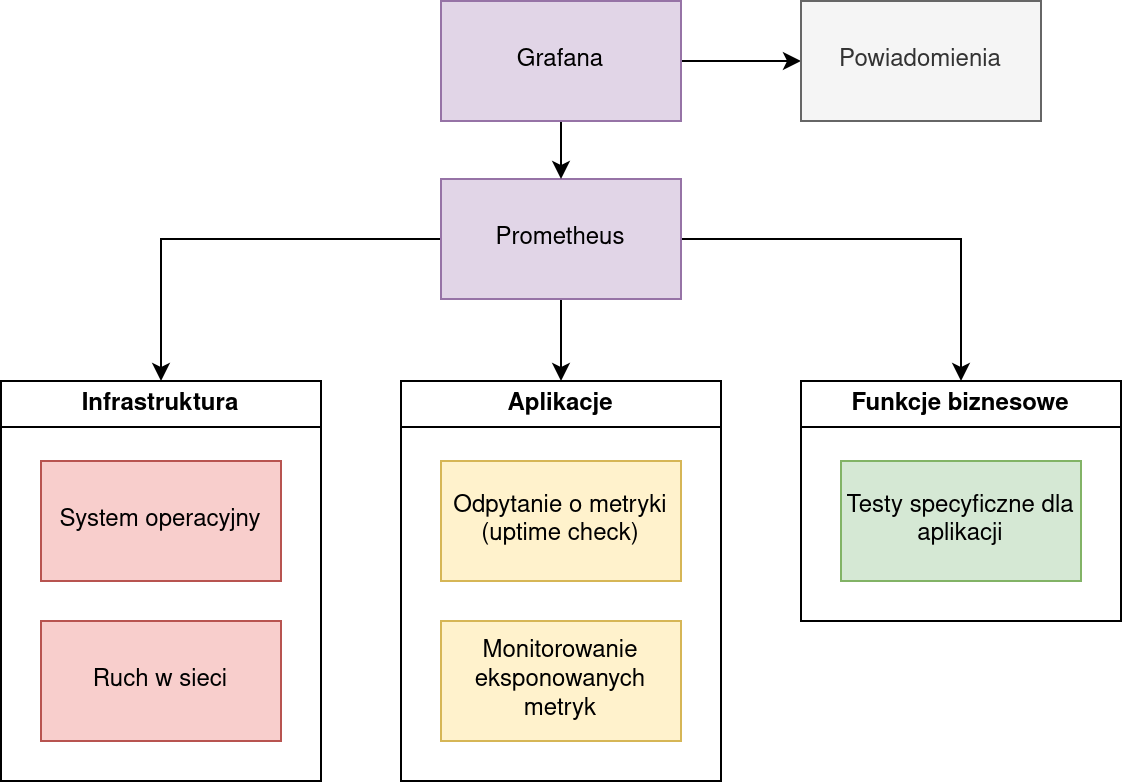
\includegraphics[width=0.8\linewidth]{infra.png}
    \caption{Monitoring infrastruktury na serwerze prywatnym.}
  \end{figure}
\end{frame}

\begin{frame}
  \frametitle{Przykład -- monitorowanie własnej infrastruktury}
  \begin{figure}
    \centering
    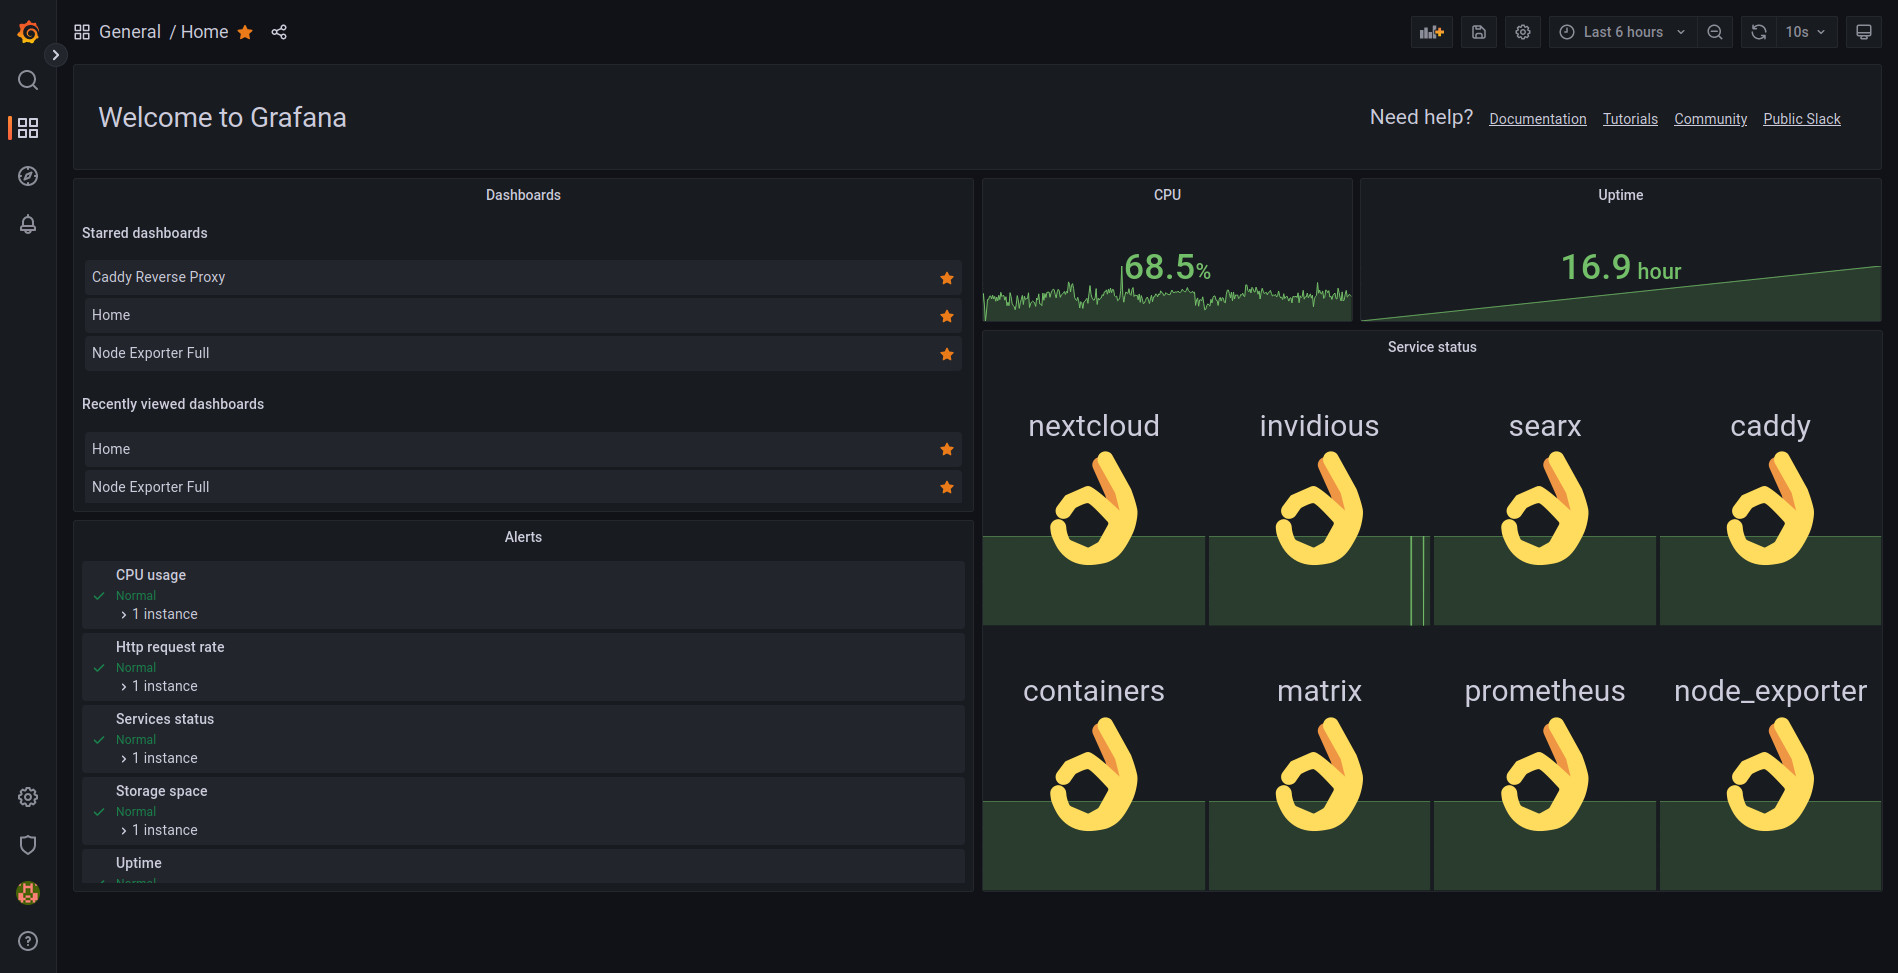
\includegraphics[width=1.0\linewidth]{grafana_dashboard_main.jpg}
    \caption{Główny panel Grafany -- ogólny podgląd stanu infrastruktury.}
  \end{figure}
\end{frame}

\begin{frame}
  \frametitle{Przykład -- monitorowanie własnej infrastruktury}
  \begin{figure}
    \centering
    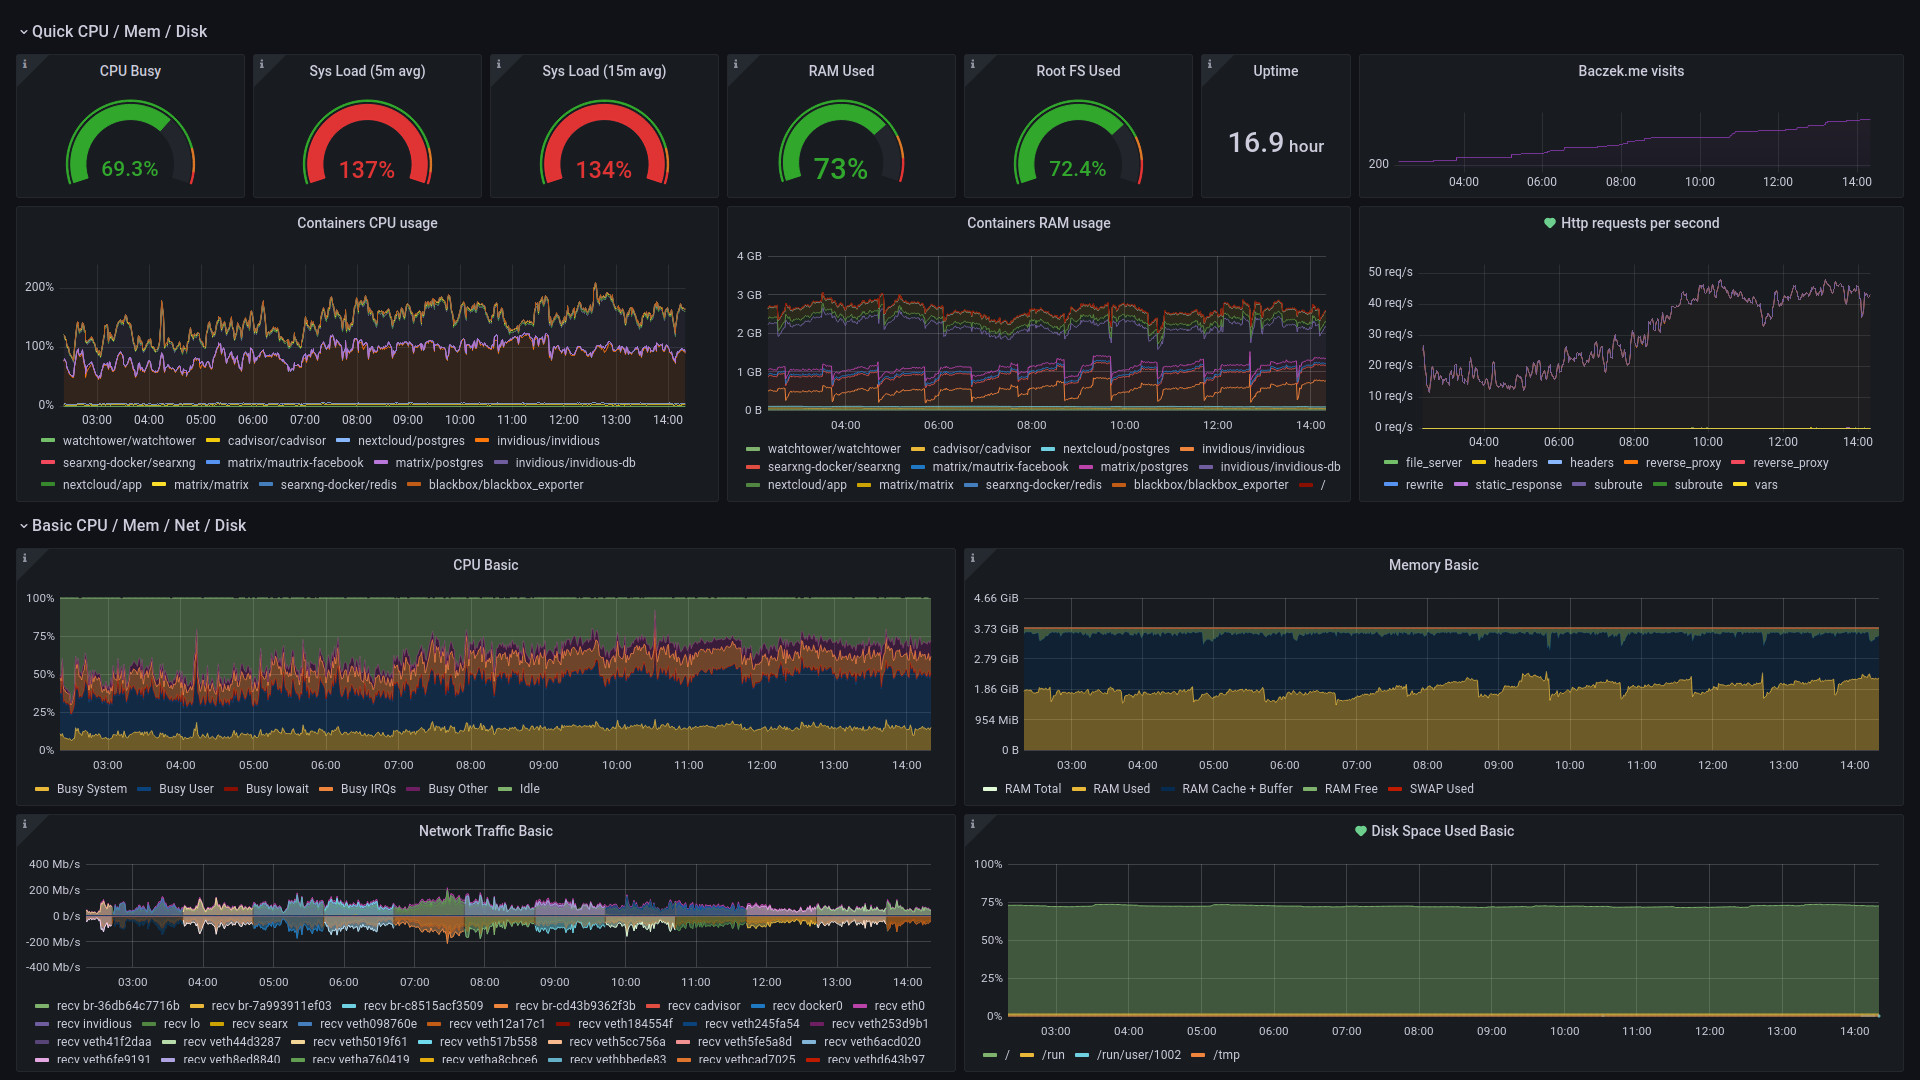
\includegraphics[width=1.0\linewidth]{grafana_node_exporter.jpg}
    \caption{\textit{Prometheus Node Exporter} - podgląd metryk systemu operacyjnego.}
  \end{figure}
\end{frame}

\begin{frame}
  \frametitle{Przykład -- monitorowanie własnej infrastruktury}
  \begin{figure}
    \centering
    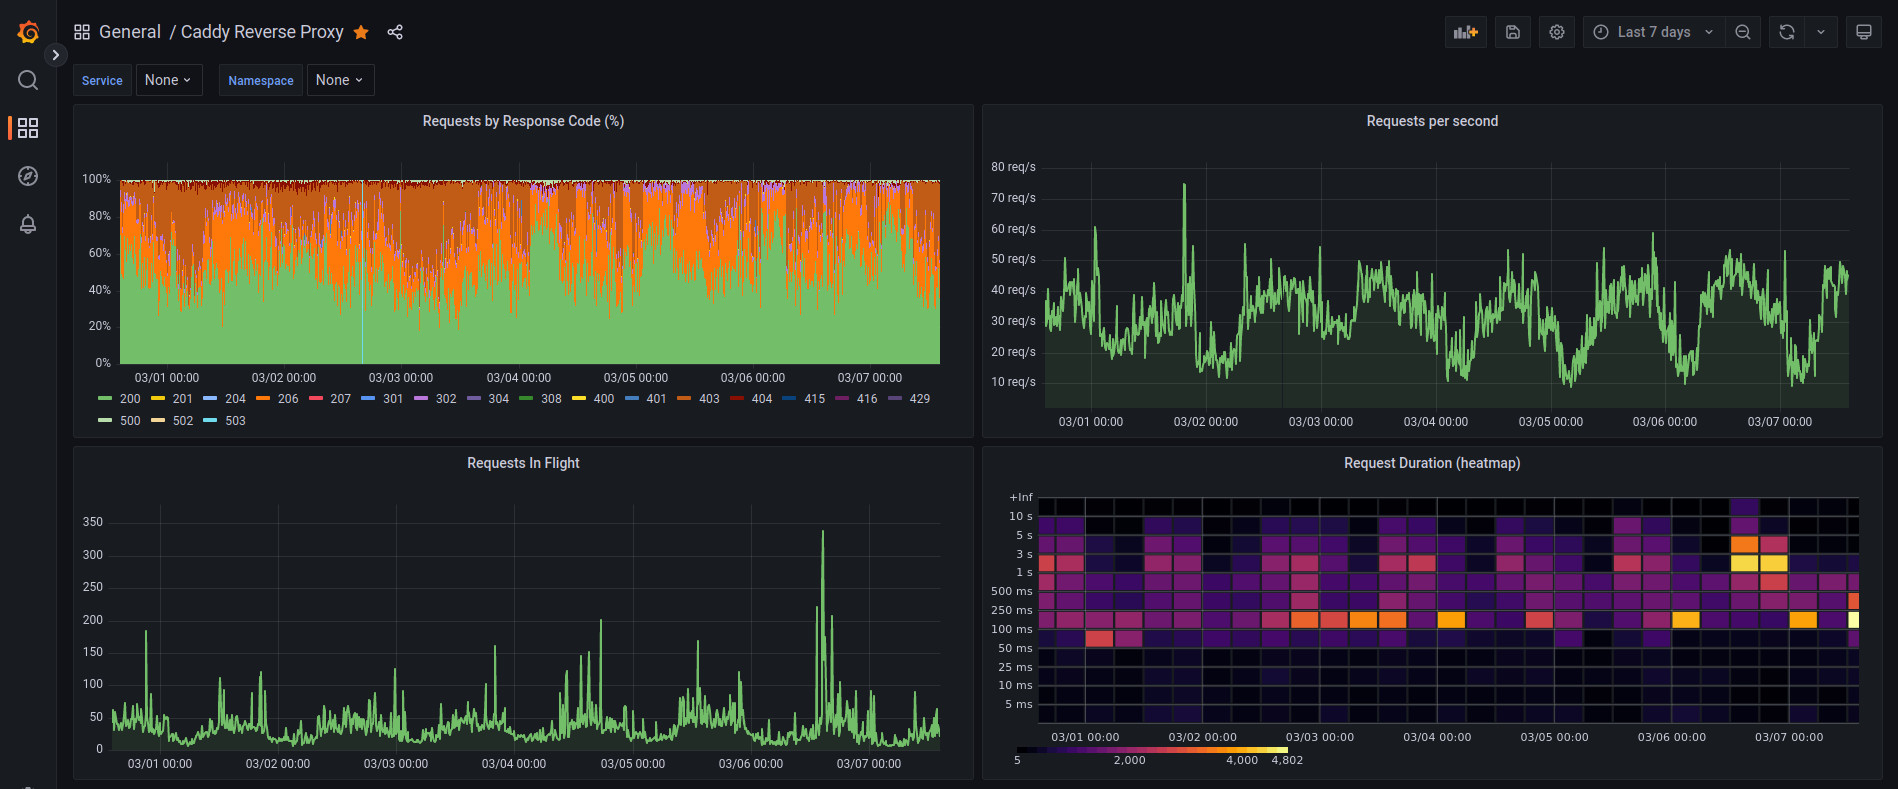
\includegraphics[width=1.0\linewidth]{grafana_caddy.jpg}
    \caption{Metryki eksponowane przez serwer webowy \textit{Caddy} (odpowiednik \textit{Apache}/\textit{NGINX}).}
  \end{figure}
\end{frame}

\begin{frame}
  \frametitle{Przykład -- monitorowanie własnej infrastruktury}
  \begin{figure}
    \centering
    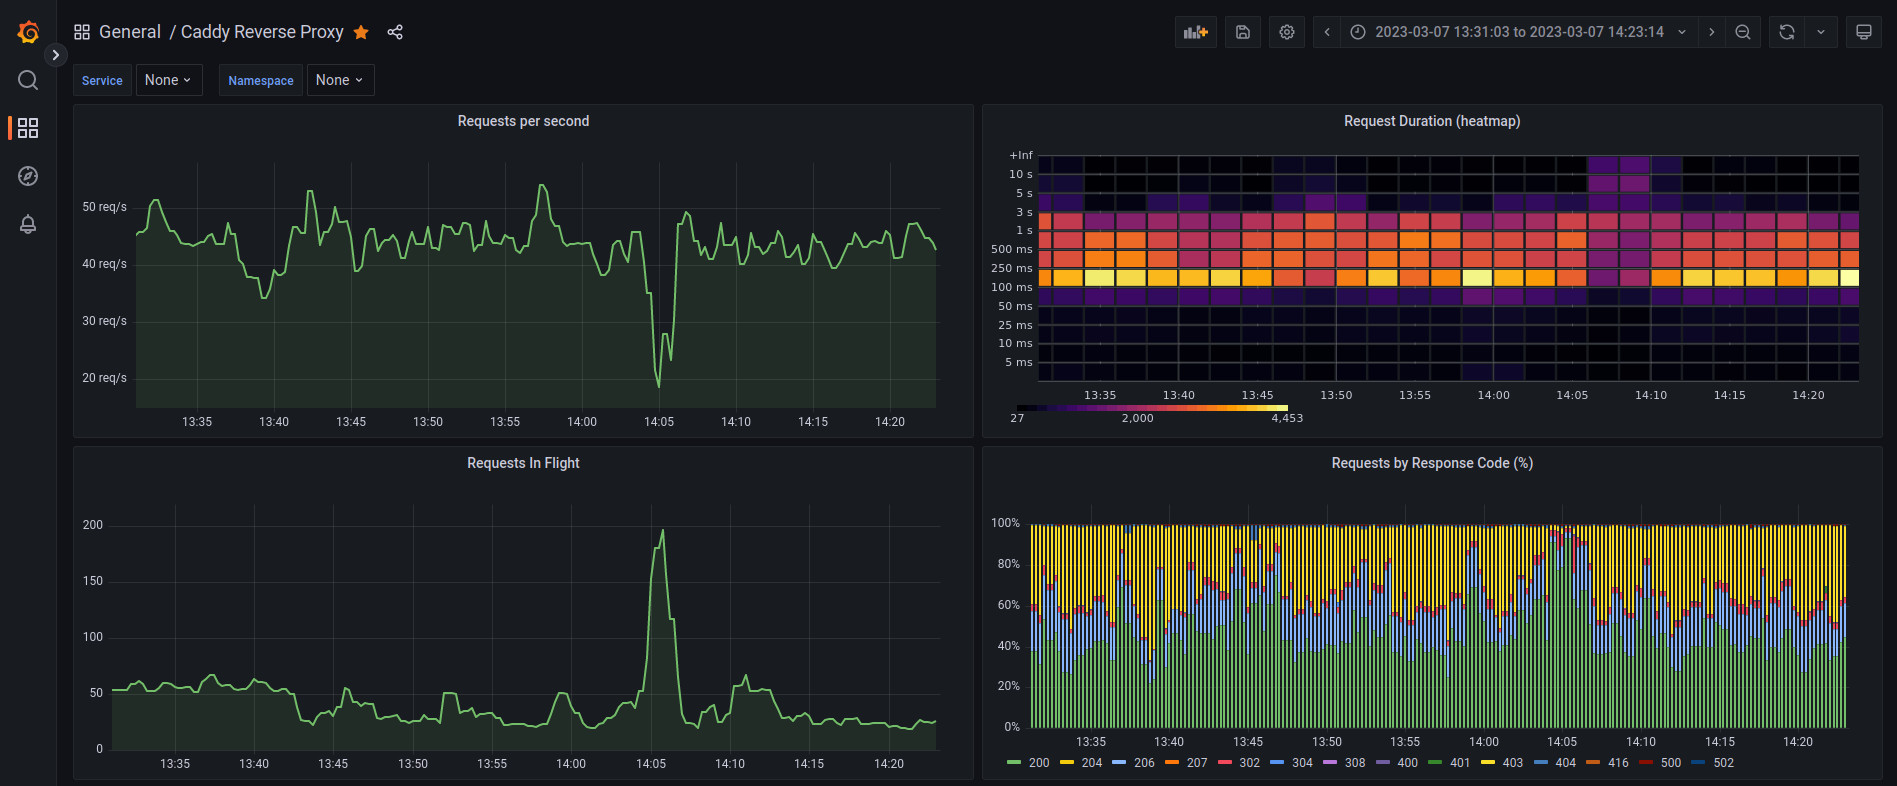
\includegraphics[width=1.0\linewidth]{grafana_caddy_example_incident.jpg}
    \caption{Przykładowy incydent w infrastrukturze - chwilowe przedłużenie czasu przetwarzania zapytań. Przykład korelacji metryk.}
  \end{figure}
\end{frame}

\begin{frame}
  \frametitle{Przykład -- monitorowanie własnej infrastruktury}
  \begin{figure}
    \centering
    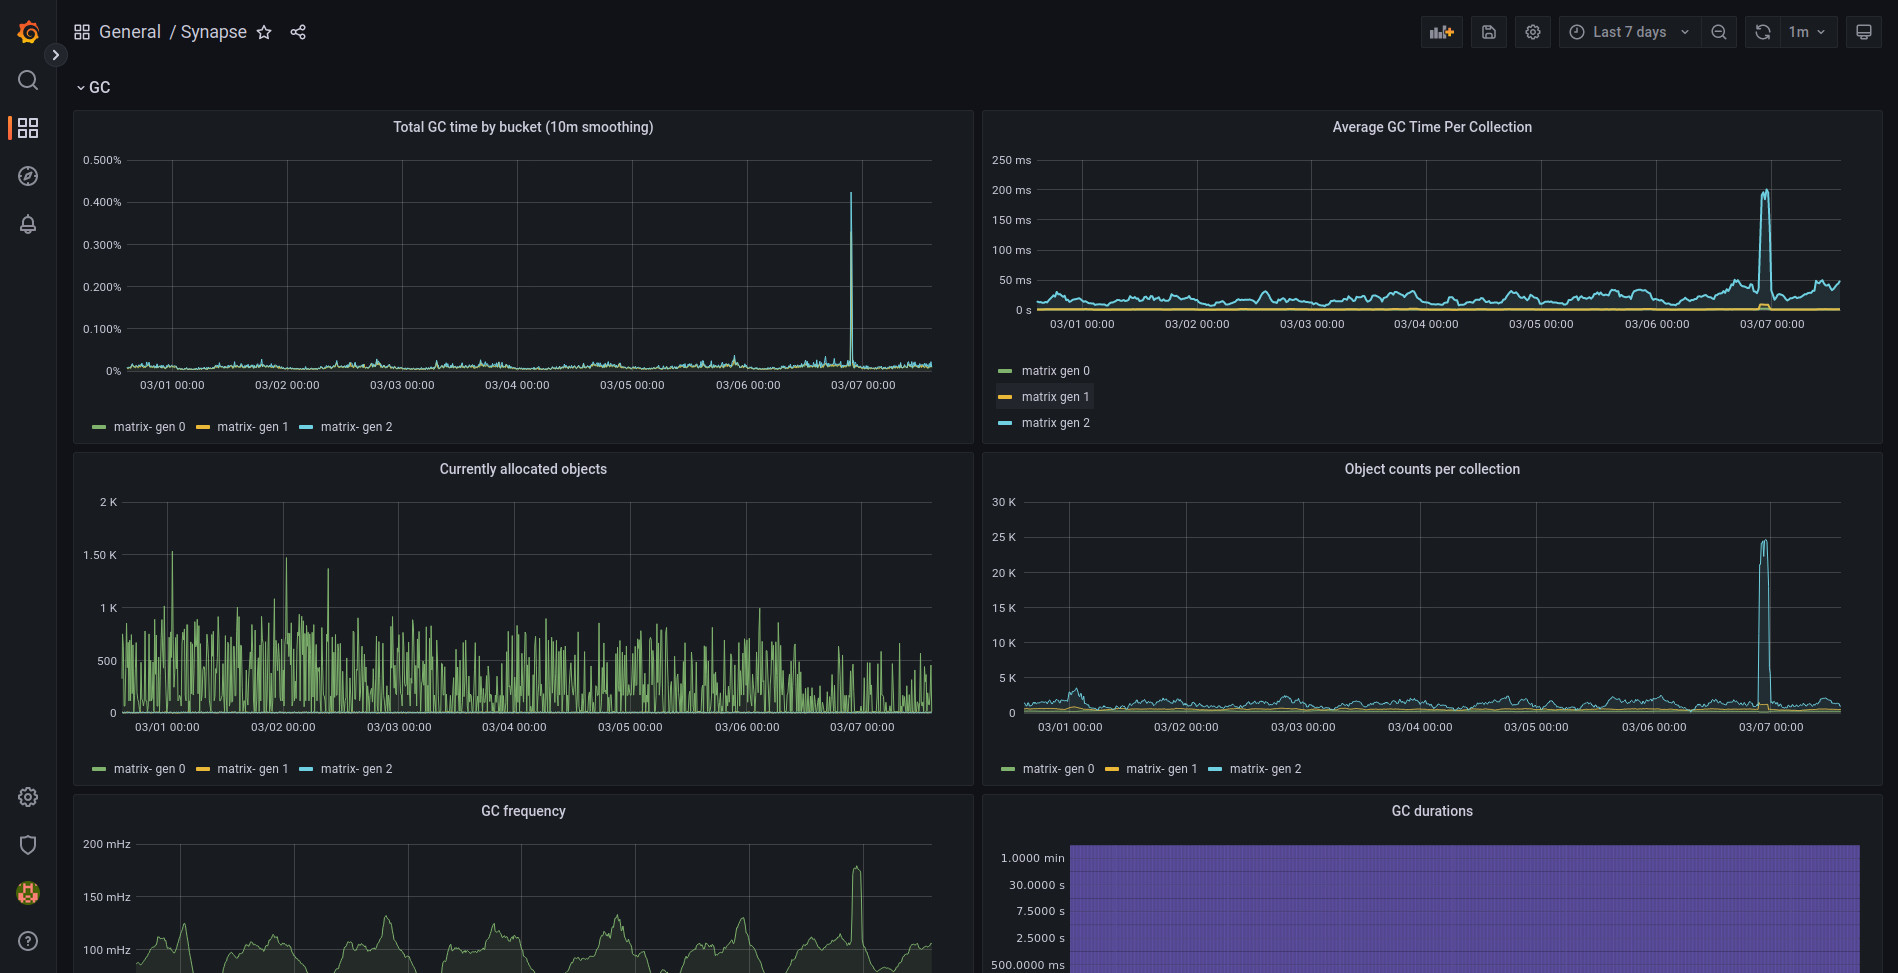
\includegraphics[width=1.0\linewidth]{grafana_matrix_python_gc.jpg}
    \caption{Metryki dotyczące \textit{garbage collectora} w aplikacji \textit{Synapse} -- serwer protokołu \textit{Matrix} napisany w języku \textit{Python}.}
  \end{figure}
\end{frame}

\begin{frame}
  \frametitle{Monitorowanie już na poważnie}
  \begin{figure}
    \centering
    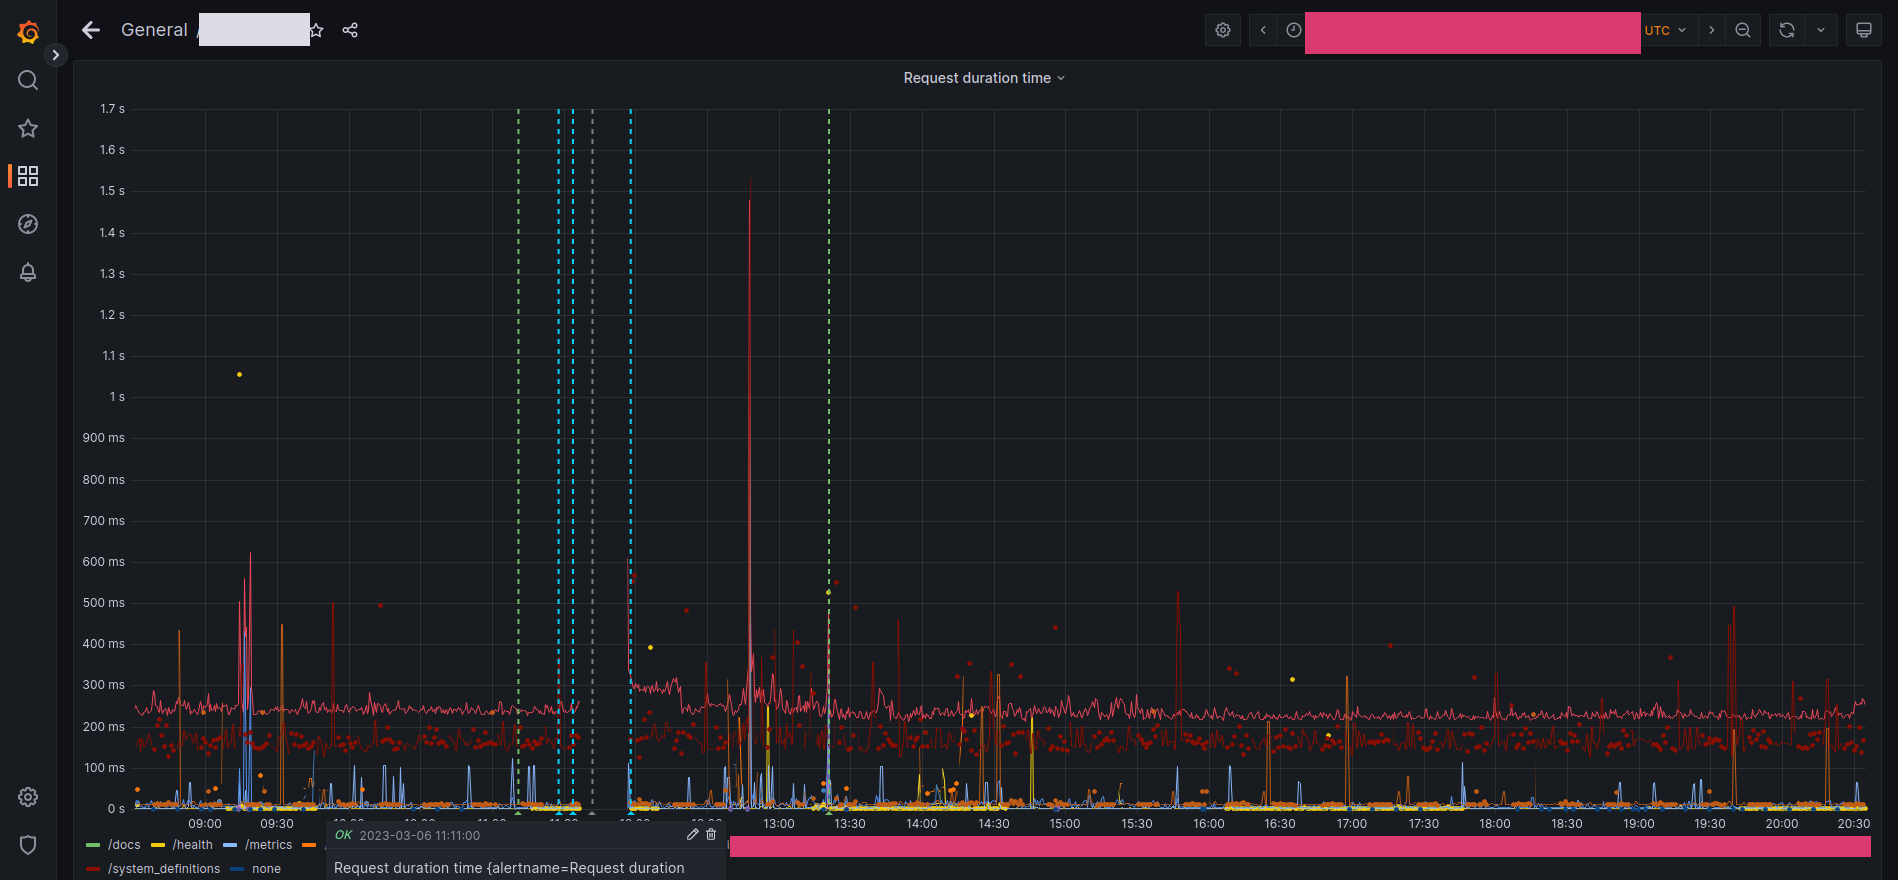
\includegraphics[width=1.0\linewidth]{grafana_request_duration_incident_example.png}
    \caption{Zapis występowania alertów na panelu monitorującym czas przetwarzania zapytania w API.}
  \end{figure}
\end{frame}

\section{Podsumowanie}

\begin{frame}
  \frametitle{\textit{Applied Observability} -- podsumowanie}

\begin{multicols}{2}

  \begin{enumerate}
    \item \textbf{Niski koszt} wprowadzenia,
    \item szeroki wybór \textit{open-source'owych} narzędzi,
    \item \textbf{duży wzrost zrozumienia} budowanego/hostowanego produktu,
    \item powiadomienia o awariach,
    \item automatyczne reagowanie na incydenty.
    \item dane pozwalające na \textbf{wykonywanie decyzji} technicznych i biznesowych.
      % \begin{enumerate}
      %   \item technicznych,
      %   \item biznesowych.
      % \end{enumerate}
  \end{enumerate}

  \begin{figure}
    \centering
    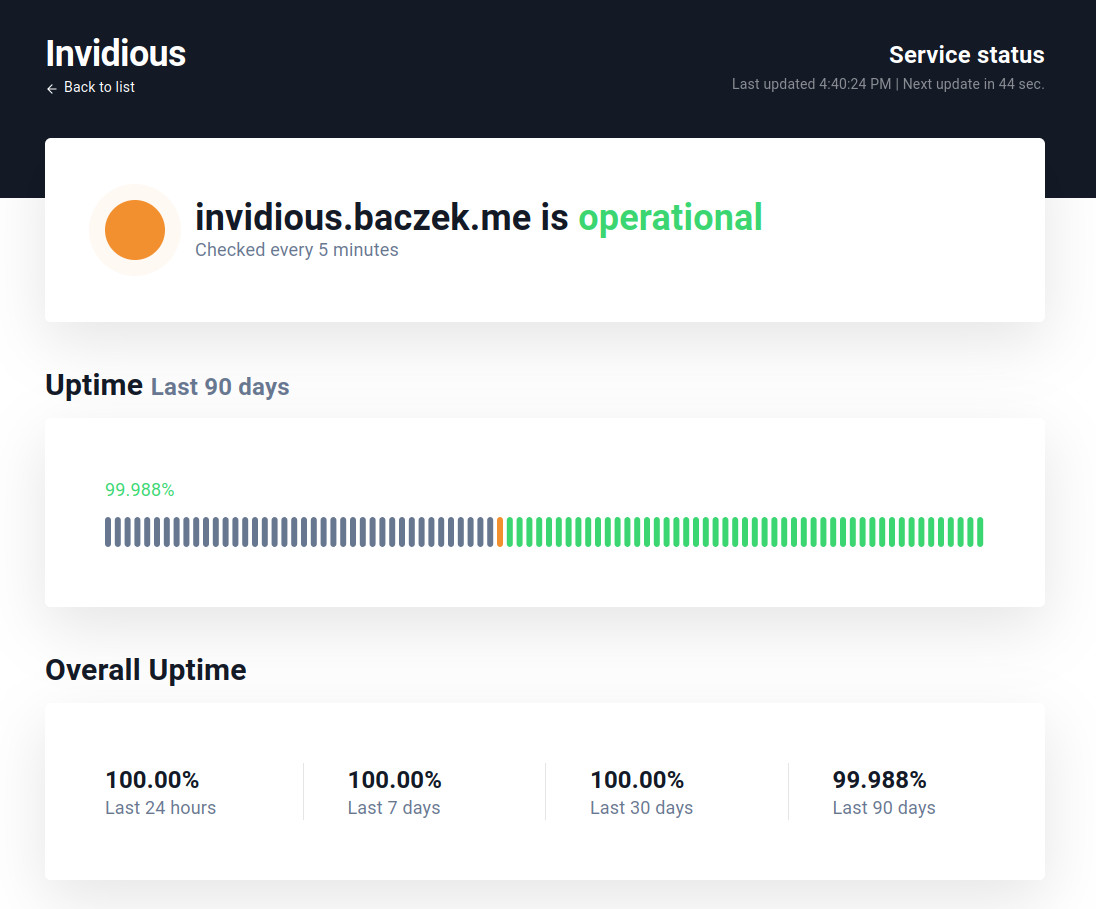
\includegraphics[width=1.0\linewidth]{invidious_uptime.jpg}
    \caption{Statystyki dostępności usługi \textit{Invidious}, hostowanej i monitorowanej w ramach własnej infrastruktury.}
  \end{figure}
\end{multicols}

\end{frame}

\section{Bibliografia}

\begin{frame}
  \begin{thebibliography}{99} % Beamer does not support BibTeX so references must be nserted manually as below
  \bibitem[Pourmajidi, 2023]{ibm} Pourmajidi, William and Zhang, Lei and Steinbacher, John and Erwin, Tony and Miranskyy, Andriy (2023)
  \newblock A Reference Architecture for Observability and Compliance of Cloud Native Applications
  \newblock \emph{Toronto Metropolitan University, University of Maryland, Baltimore County, USA, IBM Canada Lab, Toronto, Canada, IBM Cloud Platform, Austin, USA}
  \newblock \url{https://www.gartner.com/smarterwithgartner/how-to-start-an-it-monitoring-initiative}

  \bibitem[Perri, 2022]{gartner} Lori perri (2022)
  \newblock Monetizing Observable Data Will Separate the Winners and Losers
  \newblock \emph{Gartner Insights}
  \newblock \url{https://gartner.com/en/articles/monetizing-observable-data-will-separate-the-winners-and-losers}

  \end{thebibliography}
\end{frame}

\begin{frame}
  \begin{thebibliography}{99} % Beamer does not support BibTeX so references must be nserted manually as below
  \bibitem[Shetty, 2017]{gartner2} Sony Shetty (2017)
  \newblock How to Start an IT Monitoring Initiative
  \newblock \emph{Gartner Insights}
  \newblock \url{https://www.gartner.com/smarterwithgartner/how-to-start-an-it-monitoring-initiative}

  \end{thebibliography}
\end{frame}

\end{document}

